\documentclass[conference]{IEEEtran}
\IEEEoverridecommandlockouts
% The preceding line is only needed to identify funding in the first footnote. If that is unneeded, please comment it out.
\usepackage{cite}
\usepackage{url}
\usepackage{amsmath,amssymb,amsfonts}
\usepackage{algorithmic}
\usepackage{graphicx}
\usepackage{textcomp}
\usepackage{xcolor}
\def\BibTeX{{\rm B\kern-.05em{\sc i\kern-.025em b}\kern-.08em
    T\kern-.1667em\lower.7ex\hbox{E}\kern-.125emX}}
\begin{document}

\title{Modifying Existing Multiplayer Games Using Blockchain: Crypto-Craft}
\author{\IEEEauthorblockN{Callum Smith}
\IEEEauthorblockA{\textit{School of Information Systems} \\
\textit{Queensland University of Technology}\\
Brisbane, Australia \\
csmit863@outlook.com}
}

\maketitle

\begin{abstract}
Existing multiplayer games serve as useful low-stakes playgrounds for experimenting with blockchain technology and economic systems. This demo presents the development of a prototype blockchain-enabled Minecraft server that allows game items to be tokenized and exchanged through use of in-game commands. The system leverages popular decentralized exchange (DEX) infrastructure, automated market maker (AMM) mechanics and a custom server plugin that bridges in-game assets to on-chain ERC-20 tokens. Crypto-Craft serves both as a research prototype for blockchain-enabled game economies and as a hands-on educational platform for understanding decentralized finance (DeFi), tokenization, liquidity dynamics, and market behavior.
\end{abstract}

\begin{IEEEkeywords}
Decentralised Financial Services,
Token Economy,
Blockchain for Metaverse and Digital Twins
\end{IEEEkeywords}

\section{Introduction}
Minecraft is a widely recognized game with an expansive and flexible world, making it a strong candidate for educational and experimental applications \cite{unisa2025minecraft}. 
The primary goal of this project, called Crypto-Craft, is to help players understand DeFi concepts through direct interaction within a familiar game environment.

This demo introduces a blockchain-based economy implemented as a Minecraft server plugin. The system enables in-game items to be tokenized and exchanged using on-chain ERC-20 tokens and DEX mechanisms. 
By leveraging AMM models and existing DEX infrastructure, players can mine, trade, and manage digital assets without needing prior knowledge of blockchain wallets or development tools.
The project contributes:
\begin{enumerate}
\item an experimental sandbox for studying AMM-driven game economies,
\item a practical architecture for managing in-game assets,
\item a foundation for future research on blockchain-based multiplayer systems.
\end{enumerate}

\section{Rationale and Contribution}

\subsection{Choice of Game Environment} 
Minecraft is an easily modifiable and open-ended game world that enables complex player interactions. Modifications can be made to the server software enabling players to use custom commands, including interacting with a blockchain, without the need for players to download extra software. The game world contains finite resources, given a world border is set. Some items in the game world are more rare than others, and have different utilities. Players often have different motivations to one another, sometimes overlapping. This enables the introduction of a dynamic economy and supports empirical observations, given there are enough players\cite{butler2024minecraft}. The relatively simple gameplay loop of collecting resources and constructing buildings or items should provide the supply and demand necessary for the economy to function. 

\subsection{Economy and Blockchain Justification}
In larger, more advanced server setups, players typically have demands for economy functionality to introduce new objectives, increase competition, add new goals or stimulate interaction between players. Unlike traditional game economies backed by centralized databases, the use of blockchain enables verifiable ownership, cross-server interoperability, and composability with external financial systems. A blockchain provides an immutable, globally accessible state, meanwhile smart contracts introduce a layer of programmability\cite{ethereumevm}. 

Players are able to interact with the same blockchain economy over multiple Minecraft servers and worlds, so long as the plugin is configured to point to the same smart contracts and network. This allows for a parallelised game world, which can lighten server load while keeping players engaged with each other. Since the economy is blockchain based, it makes the in-game economy highly extensible and could potentially allow client-defined features such as in-game factions, trading rules, out-of-game trading, out-of-game activity logs and potentially DAOs. Eve Frontier makes heavy use of this extensibility property with their in-game Smart Assembly system\cite{evefrontiercontracts}. 

\subsection{Education}
As a topic of learning, blockchain is challenging due to its multidisciplinary nature. Teaching blockchain within the confines of a game world promotes curiosity from players to investigate the inner workings of particular blockchain mechanisms which may be relevant or beneficial for them to understand. Further, making an easy to use UI, particularly one based inside of a game, allows players to interact with a blockchain without the heavy technical setup.


\section{Demo Description}
A Minecraft server is hosted to enable multiplayer gameplay with the plugin enabled. This allows players to join without downloading any extra software other than the game itself. Upon joining, a wallet and keypair is automatically created and registered to that user in backend storage. While this provides frictionless onboarding of players, server-side custody remains a problem to be addressed in a future iteration of this project.

Once in the game world, the player can immediately start mining blocks and using the "/sell (item)" command to sell items in their inventory in exchange for "Blockcoins" at the market price. Behind the scenes, the market price is retrieved from a Uniswap V2 pair contract containing an ERC20 tokenised version of the item as well as ERC20 Blockcoins. The initial liquidity of this pair contract is seeded by a special server administrator wallet which controls the creation and redemption of tokenised items. Upon successfully selling an item, the player will receive Blockcoins into their registered wallet and be able to check their balance via "/balance". Buying and selling items dynamically adjusts the price thanks to the automated market maker mechanisms behind Uniswap V2. Players can check the changing prices of items from using "/price (item)".

Players can send Blockcoins to each other using the "/send (player) (amount)" command which triggers a transfer from the sender to the receiver's wallet of Blockcoins. To introduce utility for Blockcoins as well as scarcity for items, a worldborder was set which can be expanded by paying Blockcoins via "/expand (distance)". 
All these blockchain transactions occur without requiring the player to seed their wallet with ether, connect their blockchain wallet or approve transactions; users simply type the command in-game. While this does mean that the server administrator must sponsor the transactions, it makes the gameplay experience much smoother. Since the economy uses blockchain, players can log onto other servers which use the plugin and access the same Blockcoin balance, allowing for the seamless expansion of a multi-server economy.

\section{Implementation}

\subsection{Smart Contracts}
The Uniswap V2 AMM system was used to implement a DEX due to its relative simplicity and documentation\cite{uniswapv2overview}\cite{uniswapbriefcase}. Since there would need to be potentially hundreds of items, an ERC20 factory contract, AssetFactory.sol, was created to automatically produce tokenized items as needed. The factory contract deploys modified ERC-20 contracts with owner-restricted mint and burn functionality and maintains an index of all created asset tokens. The need for a single server-wide currency "Blockcoin" was identified as the Uniswap V2 pool system is based on the AMM system, requiring two tokens to be deposited into a pool smart contract which would set the price between two tokens as well as facilitate exchange. 

\subsection{Server Plugin and Commands}
The plugin contained the functionality for translating player commands into blockchain transactions. Sometimes these commands would encompass multiple on-chain transactions. For example, initial liquidity would need to be seeded by the administrator in order to set a starting price for items. Additionally, tokenized items could not be created until a player sold an item in-game. Similarly, items could not be purchased until at least one was sold. This keeps the supply of all items tied to the in-game world instead of being artificial and functions similarly to real-world asset provisioning\cite{ethereumrwa}. 

\begin{figure}[t]
    \centering
    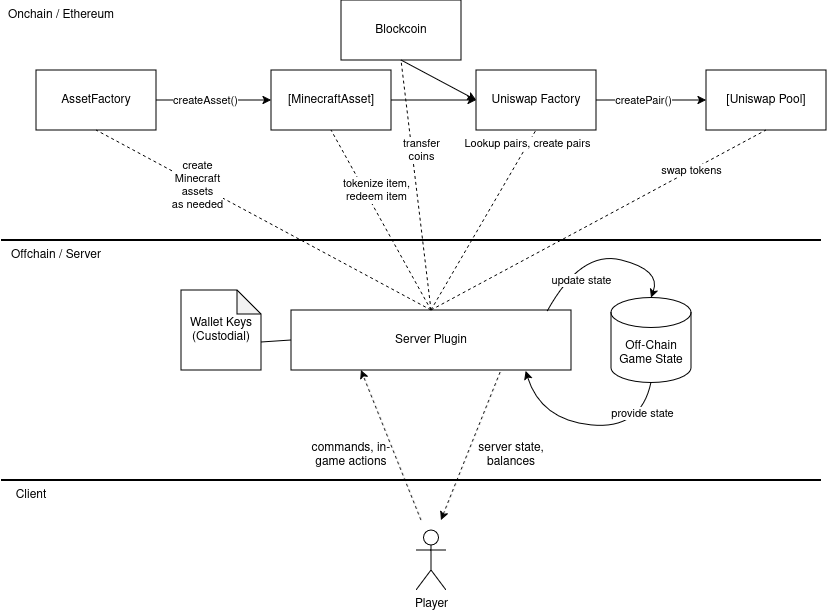
\includegraphics[width=1\linewidth]{cryptocraft_architecture.png}
    \caption{Interaction between smart contracts, plugin and client.}
    \label{fig:placeholder}
\end{figure}

\section{Evaluation}
\subsection{Gameplay}
The server was hosted on free server hosting infrastructure, a mixture of cloud and self hosted. As expected, the initial seeding of liquidity resulted in an early game rush to discover as many items as possible, in order to accumulate Blockcoins. Players learned concepts such as slippage, liquidity, and discovered various strategies such as hoarding, "dumping" items, item-hunting, world expansion, and isolation to hoard coins. Some objectives of players arose, such as coin accumulation and the attempt to "corner" certain markets. 



\subsection{Security and Threat Model Limitations}
In order to create a prototype, there were limitations in the degree of decentralisation of the Crypto-Craft project. While the blockchain economy is decentralised and uses decentralised protocols such as Uniswap, the management of player wallets is still done server-side as our focus was not on making a paired client implementation. In the future, a client could be developed which could either securely manage keys directly, or allow for a third-party wallet connection. This would also serve as an important primitive in enabling better cross-server economies.

Another security assumption made for the creation of a prototype was the use of an administrator account, which would be used by the server software to manage burning and minting tokenised Minecraft assets and other blockchain related administrative duties. While this generally works, it would be more secure if assets could be managed by a treasury body or DAO, with delegated authorities given permission to mint Minecraft assets. Further, server logs could be cryptographically audited to ensure that no admin commands have been used to summon items which were not already in the game world.

While these security risks are not acceptable for a production implementation, they allow for the demonstration of a prototype concept and can still be used in an educational context. 


\subsection{Further Improvements, Research and Applications}
Without incentives or functionality to add liquidity, the economy became impacted by large buy and sell orders. More players would make the economy more competitive and reveal the true dominant strategies of gameplay, which may provide valuable insights for future economic experiments. The system should be deployed on a live Layer 2 blockchain with high throughput to introduce real prices to items to investigate the impact on gameplay. ERC1155 would improve gas efficiency for the amount of tokens present. 

The system can potentially have a game economy state which spans multiple game worlds, run by many administrators which may or may not trust one another. For example, in a future iteration of Crypto-Craft, the game state itself may be recorded using smart contracts to verify that separate server instances are being run correctly. This type of setup could allow a single game world to be "massively online"\cite{evefrontiercontracts} with tens of thousands of players. 

Beyond improvements to the project itself, this demonstration may provoke further research questions such as:
\begin{enumerate}
\item Can blockchain-based game economies teach us how real life digital economic systems can work?
\item What are the effects of introducing tokenisation and market-based pricing to in-game resources that were previously non-tradable or fixed in value?
\end{enumerate}



\section{Conclusion}
Crypto-Craft demonstrates an exploration into the use of game worlds for both economic experimentation and as tactile education tools. Future work will focus on non-custodial wallet integration, improved liquidity design, and scalable deployment on high-throughput blockchain networks.

\bibliographystyle{IEEEtran}
\bibliography{bibliography}

\end{document}